\documentclass[twocolumn,10pt]{asme2ej}

\usepackage{graphicx}
\usepackage{epsfig}
\usepackage{epstopdf}
\title{Sign language synthesis from Natural Language Processing}


\author{Nijat Mursali
\affiliation{
Department of Artificial Intelligence and Robotics\\
Sapienza University of Rome\\
}}

\begin{document}

\maketitle    

%%%%%%%%%%%%%%%%%%%%%%%%%%%%%%%%%%%%%%%%%%%%%%%%%%%%%%%%%%%%%%%%%%%%%%
\begin{abstract}
{
{\bf Abstract}—Sign language is a visual language that individuals with speech and hearing impairments use to communicate in their daily conversations. It is entirely an optical communication language due to its native grammar, which differs fundamentally from that of spoken languages.
The fundamental purpose of this paper is to describe the algorithm which takes the spoken language from the user, recognize word(s) with an algorithm and convert words to sign language. As an output, we display the images with the sign language. 
}
\end{abstract}

\section{Introduction}

There are more than 7000 known living languages in the world divided in 136 different language groups. Among these 136 language families, Sign language is one and this family contains 136 sign languages all over the world depending upon the region of the world. Sign language is used by hearing impaired people to convey their message. 

Sign language is a nonverbal language used by the deaf and hard of hearing to communicate using hand shapes, facial expressions, gestures, and other areas of the body. Because sign languages lack a well-defined structure or grammar, they have no or very little acceptance outside of their limited community. Approximately 72 million of the world's nearly 7 billion inhabitants are deaf or hard of hearing. Out of such a large population, roughly 4.3 million utilize Sign language. The remaining roughly 67 million deaf and hard of hearing persons do not communicate using any sign language. As a result, over 90% of the deaf have extremely limited or no access to schooling and other information. 

In the following paragraphs we will be discussing how we developed the application that is capable of getting the speech from the user and giving the images of the sign language as output.

\section{Motivation}

A good Sign Language Recognition (SLR) system can break down the barriers that exist between the speech and hearing communities and the speaking culture. The objective of SLR is to create methods and methodologies for correctly recognizing a series of gestures and understanding the meaning of the gestures. SL presents a problem in that it is multi-channel, interpreting meaning in several ways at the same time.

SLR is a difficult and motivating work because to several restrictions and variables. This is not easy task to accomplish because there are not always exact phases we can use to convert to ASL. Thus, we had to think of a way to handle the dataset and accomplish the task. 

\section{Data collection}

Data gathering is an essential component of research in all fields of study, including the sciences, social sciences, technology, humanities, and business. Methods for data collecting may differ per discipline, but the emphasis on ensuring exact and genuine collection leftovers always the same.

We have created a new dataset of ours by gathering the sign language images from different sources. The fundamental source was to use some phases which gave us the opportunity to get images of sign language for different words. In order to parse all the images manually would not be a good idea, thus we have created a new function in order to call the links automatically and parse the images from all of those links. We have used {\emph BeautifulSoup} for this and for all the letters in English language (A-Z) we have checked every single link for the images and added them to local storage. 

\begin{figure}[h]
    \centering
    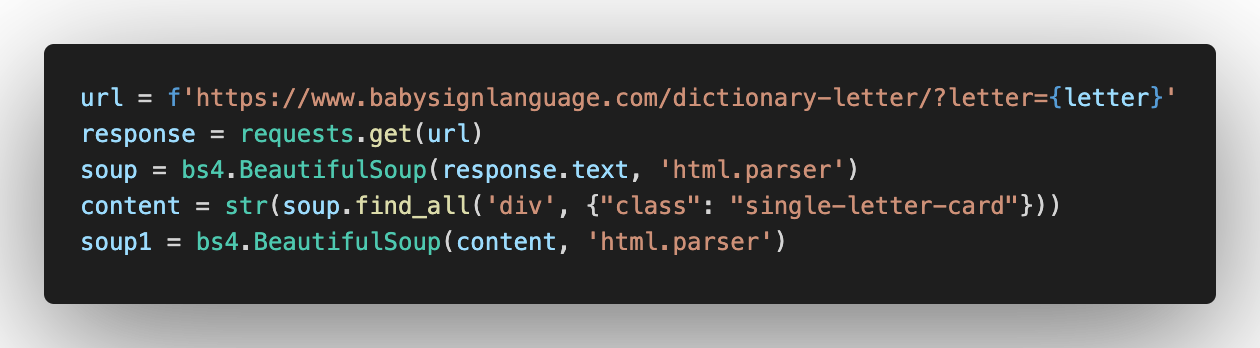
\includegraphics[width=0.5\textwidth]{figure/fig1.png}
    \caption{Getting the links for all letters}
    \label{fig:mesh1}
\end{figure}
As shown in the image, we have first added all the alphabet letters in English language and for those letters, we have checked the URL response and for specific element we get all the links. Then we have added those links to the list for further processing. 

Then, for all the links, we are making the GET request for specific elements where images are added by their source and name. Then, within the loop, we are making the request to get the images and add them to the local storage. 

\section{Development}

\subsection{Interface}

Before moving to sign language, we need to discuss how we built the structure of the application. We have used the {\emph Tkinker} which is a Python binding to the Tk GUI toolkit. It is the standard Python interface to the Tk GUI toolkit, and is Python's de facto standard GUI. We have created a simple interface where the user can click the button to get the speech from the user and then the algorithm will check which words the user has said. The following image shows the interface of the application.

\begin{figure}[h]
    \centering
    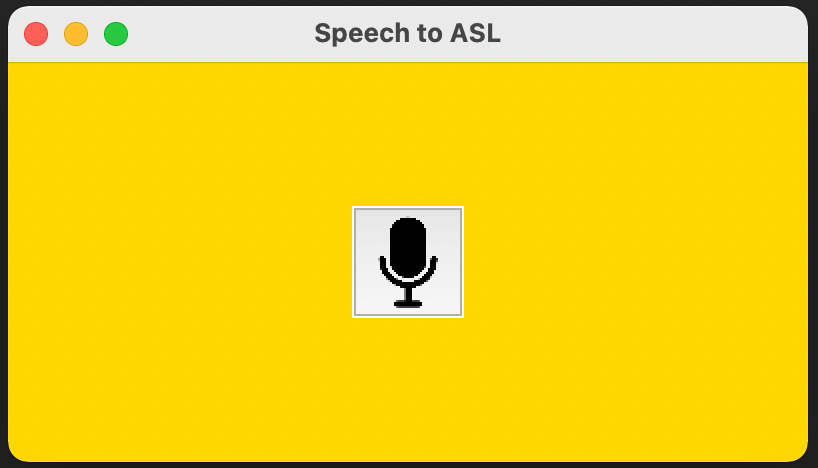
\includegraphics[width=0.4\textwidth]{figure/fig2.png}
    \caption{Getting the links for all letters}
    \label{fig:mesh1}
\end{figure}

In order to get the input from the microphone, you need to press the microphone button. After pressing the button, the input is recorded and added to a variable called "text". 

\subsection{Algorithm}

As we have explained earlier, we managed to get around 1000 images for our dataset by applying our code from scratch. The fundamental idea for this part was to add all the alphabetical letters in English (A-Z) and checking the URL for all those letters in a loop. For each of those letters, we check if the content contains the special element. If yes, we added the href (an attribute of the anchor tag) elements to the list. For the next step, in a loop for each element of that list, we have checked if the link contains the image tag. If yes, we have used PIL library to resize and save the images to local system. 

The fundamental step for the algorithm part was the base of the code where we first got the sentences from the user. As we explained, we used microphone in order to get the input from user and by using the Google Speech API we managed to add the speech to text variable. As we store the text variable (which is a string), we then moved to NLTK where we divided the sentence into words by tokenizing them. 

In the following process, we use NLTK which is a suite of libraries and programs for symbolic and statistical natural language processing for English written in the Python programming language. This library is basically we can use to simulate NLP. We use {\emph "word tokenize"} from NLTK library to get the tokenized words. Tokenizing allowed us to easily break up text by word or phrase. Then it allowed us to deal with smaller chunks of text that are still pretty cohesive and intelligible even when taken out of context. It was the initial stage in transforming unstructured data into structured data that could be analyzed more easily. Normally, there are two ways to tokenize: word and sentence. In our case, we have used word tokenize because we needed to deal with simple sentences. 

For this process, we also check if sentences have some punctuations. As we know, in English language {\emph '} is used so often, for instance "don't". When we use NLTK library, it divides word by "do" and "n't" because it understands "n't" is a contradiction of "not". Thus, we just removed the punctuations. Another fundamental step was to check the stopwords. Stop words are words that you wish to ignore, so while you're processing text, you filter them out. Because they don't contribute much sense to a sentence, common words like 'in,' 'is,' and 'an' are frequently employed as stop words. We have then added a new empty list and by checking the stop words in the sentence we add the important words to our list and check for next steps. 

Another step for NLP part was to use stemming for our algoritm. Stemming is a text processing task in which you reduce words to their root, which is the most important element of the term. For example, the roots of the words "helping" and "helper" are the same. Stemming helps you to focus on the fundamental meaning of a word rather than the specifics of how it is used. There are other stemmers in NLTK, but you will be utilizing the Porter stemmer. After checking the stopwords, we have used Porter's stemmer in order to bring the words to their initial roots. For instance, if we say "I am going to buy flowers." if we use stemmer, the output will be "['i', 'am', 'go', 'to', 'buy', 'flower']" which brings all the words to their initial forms. 

The next step for our algorithm was to check the words and images for those words in our database. As we have mentioned earlier, we have managed to add more than 1000 words for our dataset. We know that it is not always possible to have all the words in the dataset, so for that case we are using the alphabetical characters in English language. So, basically, if a NLP tokenized sentence contains the word that is in our dataset we add that image to the list, otherwise we divide the word into characters of letters and adding image in sign language for each of those letters. 

As a final step, we have used the {\emph webbrowser} library which comes with Python to export the images to GIF file in order to display them in the new browser. For the images, we previously added all the images to the list which contains the path of all of the images in the system. Thus, by using the library, we append the images and save the images to GIF file and open the GIF in new tab by using the webbrowser. 

\section{Results}
To test the proposed work, we have taken some simple sentences from different users. For the moment, we take simple sentences with 2-5 words not to have problems with the algorithm, thus, we have taken mostly used English words and sentences into consideration.

As an example, we can say the sentence is "I wanted to go to America." In this case, if we tokenize the words, we will get the list of words which are "I", "want", "to", "go", "america". Thus, our application checks every words in the dataset, if it exists or not, so if yes, it adds the image to the list of images. If the image does not exist in the dataset for that specific word, it divides the words into characters and adds the alphabetical character of each word into the list of images. For instance, in our sentence we had "to", so we can show it as an alphabetical characters. The following figure shows the output of the sentence we have mentioned above. 

\begin{figure}[h]
    \centering
    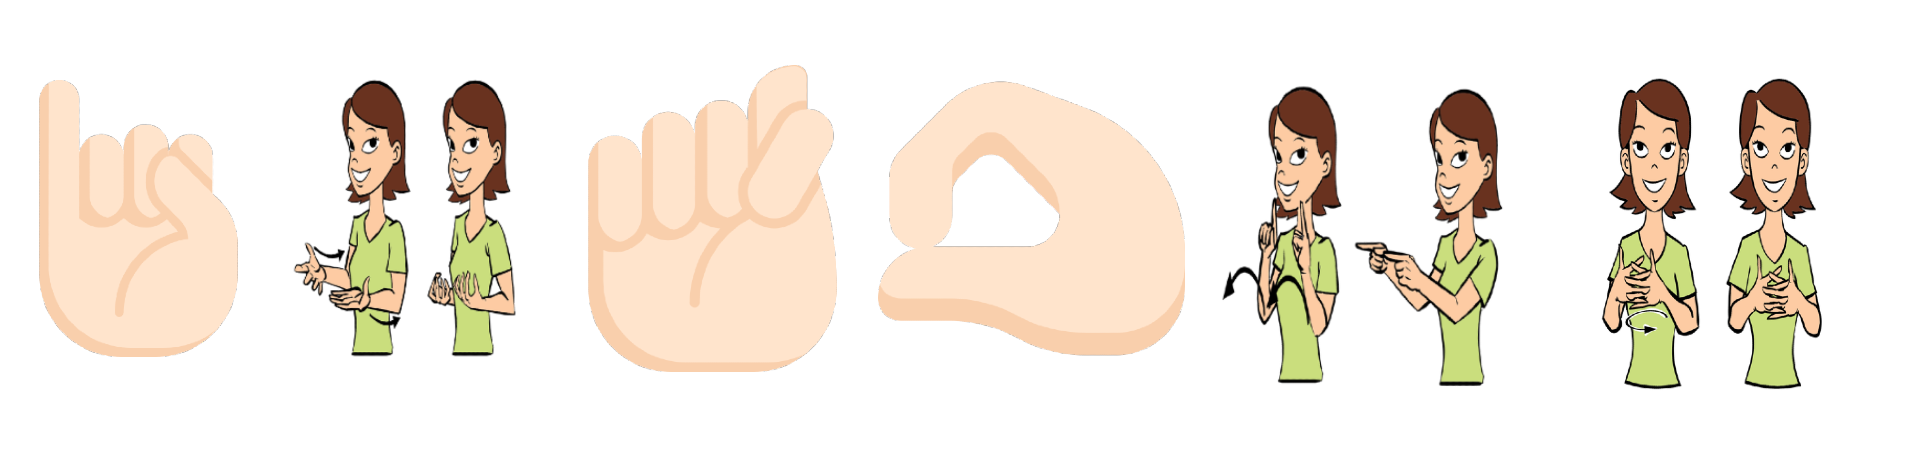
\includegraphics[width=0.4\textwidth]{figure/Untitled.png}
    \caption{Output of spoken language into ASL}
    \label{fig:mesh1}
\end{figure}

\section{Conclusions}
This research paper exhibits an optimal approach, to accomplish the algorithm which makes it possible to get the speech input from the user and apply the Natural Language Processing (NLP) to convert the words to initials forms and display the images of the words in sign language. In order to accomplish this task, we have gathered around more than 1000 images and 26 alphabet letters in English language. For the NLP, we have used specific NLTK library and algorithms to convert the words into the initial form. We also took the some specific punctuations in English language. Thus, if no word is in the database, it checks the characters of the unknown word and displays the images of letters in English alphabet.  

\section{Future work}
This research may be expanded to identify more complex sentences by adding our dataset of images which could explain the phases in English language. This research work can also be extended to recognize the video from the camera for English alphabet, words and sentences. 

\begin{acknowledgment}
I would like to thank my professor Christian Napoli for his guidance throughout this project. I would also give my huge thanks to my colleagues for testing the application and specifying the accuracyy the have got for this project. 
\end{acknowledgment}

\begin{thebibliography}{9}
\bibitem{knuthwebsite} 
American Sign Language,
\\\texttt{https://www.nidcd.nih.gov/health/american-sign-language}

\bibitem{latexcompanion} 
Ss, Shivashankara \& S, Dr.Srinath. 
\textit{American Sign Language Recognition System: An Optimal Approach. }. 
International Journal of Image, Graphics and Signal Processing. 10.
\end{thebibliography}


\end{document}
